\documentclass[11pt,aspectratio=169,usenames,dvipsnames]{beamer}
\usetheme{SimplePlus}

\usepackage{threeparttable}
\usepackage{booktabs}
\usepackage{xcolor} % For custom colors
\usepackage{tikz} % For styling enumerate numbers
\usepackage{tcolorbox} % For colored box styling
\usepackage{amsmath, amsfonts, amssymb, amsthm} % Math related
\usepackage{natbib}
\usepackage{fontspec}
\usepackage{luatexja}
\usepackage[mathscr]{euscript}

% ---------------- %
% color definition %
% ---------------- %
\definecolor{main}{HTML}{23373B}
\definecolor{pink}{RGB}{180, 50, 110}
\definecolor{orange}{HTML}{FF8000}
\definecolor{red}{HTML}{990000}
\definecolor{blue}{HTML}{004C99}
\definecolor{lightgray}{HTML}{E7E7E7}
\definecolor{gray}{RGB}{90, 90, 90}

\newcommand{\pink}[1]{\textcolor{pink}{#1}}
\newcommand{\orange}[1]{\textcolor{orange}{#1}}
\newcommand{\red}[1]{\textcolor{red}{#1}}
\newcommand{\blue}[1]{\textcolor{blue}{#1}}
\newcommand{\green}[1]{\textcolor{OliveGreen}{#1}}
\newcommand{\magenta}[1]{\textcolor{magenta}{#1}}
\newcommand{\gray}[1]{\textcolor{gray}{#1}}
\newcommand{\purple}[1]{\textcolor{purple}{#1}}
\definecolor{yellow}{HTML}{EDB120}

% \setbeamercolor{alerted text}{fg=blue}

%%% automatically add spaces into enumerate and itemize environment
\let\tempone\itemize
\let\temptwo\enditemize
\renewenvironment{itemize}{\tempone\addtolength{\itemsep}{\fill}}{\temptwo}
\let\tempa\enumerate
\let\tempb\endenumerate
\renewenvironment{enumerate}{\tempa\addtolength{\itemsep}{\fill}}{\tempb}

\usepackage{fontawesome5}
\setbeamertemplate{itemize item}{\faAngleRight}
\setbeamertemplate{itemize subitem}{\faAngleDoubleRight}

\setmainfont{Crimson Pro Light}[
  ItalicFont={* Italic},
  BoldFont={Crimson Pro Medium},
  BoldItalicFont={Crimson Pro Medium Italic}]
\setsansfont{Crimson Pro Light}[
  ItalicFont={* Italic},
  BoldFont={Crimson Pro Medium},
  BoldItalicFont={Crimson Pro Medium Italic}]

\usepackage[mode=tex]{standalone}
\usepackage{tikz}
\usetikzlibrary{decorations}
\usetikzlibrary{decorations.pathreplacing, intersections}
\usepackage{pgfplots}
\usetikzlibrary{calc,positioning}
\usepgfplotslibrary{fillbetween}
\pgfplotsset{compat=newest, scale only axis, width = 10cm}

% --------------------------- %
% Section title page with toc %
% --------------------------- %
\setbeamertemplate{subsection page}{%
    \usebeamertemplate*{section page}
}
\setbeamertemplate{section in toc}[square]
\setbeamertemplate{subsection in toc}[square]
\AtBeginSection[]{
% \sepframe
\begin{frame}[noframenumbering]{Outline}
    % \tableofcontents[currentsection]
    \tableofcontents[currentsection, currentsubsection]
\end{frame}
}
\AtBeginSubsection[]{
  \begin{frame}[noframenumbering]{Outline}
    \tableofcontents[currentsection, currentsubsection]
  \end{frame}
}

% ------------ %
% beamerbutton %
% ------------ %
\newcommand{\goto}[2]{\hyperlink{#2}{\beamergotobutton{#1}}}
\newcommand{\return}[2]{\hyperlink{#2}{\beamerreturnbutton{#1}}}
\newcommand{\extgoto}[2]{\href{#2}{\beamergotobutton{#1}}}

\hypersetup{
    pdfpagemode=UseNone,
    pdftitle = {Macroeconomics I, Lecture 1},
    pdfauthor = {Hui-Jun Chen},
    pdfsubject = {},
    pdfkeywords = {},
}
\title[Lecture 1]{Lecture 1: Introduction \\ Course and Macroeconomics}
\author[Hui-Jun Chen]{Hui-Jun Chen}
\institute{National Tsing Hua University}
\date{\today}

\begin{document}

% Title Page
\begin{frame}[plain]
    \titlepage
\end{frame}

\section{Course Plan}
\label{sec:Course_Plan}

\begin{frame}{Your Instructor}
\label{slide:Your_Instructor}
    \begin{itemize}
        \item My name is \alert{Hui-Jun Chen}, you can call me HJ for convenience.
        \item I work on \alert{Macro-Finance}, investigating issues like \alert{corporate tax reform}, \alert{housing}, \alert{used capital market}, and their macroeconomics implications.
        \item Contact Info:
        \begin{itemize}
            \item Email: \href{huijunchen@mx.nthu.edu.tw}{huijunchen@mx.nthu.edu.tw}.
            \item Website: \href{https://huijunchen9260.github.io/}{https://huijunchen9260.github.io}
            \item Course website: \href{https://huijunchen9260.github.io/MacroeconomicsIAutumn2025.html}{https://huijunchen9260.github.io/MacroeconomicsIAutumn2025.html}
        \end{itemize}
    \end{itemize}
\end{frame}

\begin{frame}{Expectation}
\label{slide:Expectation}
    \begin{columns}
        \begin{column}{0.6\textwidth}
            \begin{itemize}
                \item \textbf{Participation}: can ask question anytime during the lecture
                \item \textbf{Prerequisites}: \alert{Principle of Economics}, Basic Algebra, Some knowledge of Calculus
                \item Other rules: please refer to the syllabus
            \end{itemize}
        \end{column}
        \begin{column}{0.4\textwidth}
            \begin{figure}
                
\includegraphics[width=\textwidth]{./figures/Williamson.jpg}
                \caption{Recommended but not required textbook}
            \end{figure}
        \end{column}
    \end{columns}
\end{frame}

\begin{frame}{Course Plan}
\label{slide:Course_Plan}
\begin{itemize}
    \item \textbf{Module 1}: Measurement (Week 1)
    \begin{itemize}
        \item stylized facts about Economics growth and business cycle
    \end{itemize}
    \item \textbf{Module 2}: One-period (\alert{static}) model (Week 2-6)
    \begin{itemize}
        \item micro foundation: consumers and firms
        \item macro implication: equilibrium, efficiency, resource allocation with data
    \end{itemize}
    \item \textbf{Module 3}: Two-period (\alert{dynamic}) model (Week 8-12)
    \begin{itemize}
        \item module 2 $ + $ time: \alert{intertemporal substitution}
    \end{itemize}
    \item \textbf{Module 4}: Dynamic Programming and Asset Pricing
\end{itemize}
\end{frame}

\section{Methodology of Macro}
\label{sec:Methodology_of_Macro}

\begin{frame}{What is Macro?}
\label{slide:What_is_Macro_}
    \begin{itemize}
        \item ``\alert{Macro is a method}''
        \item Models (theory) $ + $ Data (empiric) $ = $ explanation to macro events
        \begin{itemize}
            \item without models: only \alert{correlation}
            \item without data: only \alert{imagination}
            \item \alert{Friedman's critique}: models are judged by \alert{prediction power}
        \end{itemize}
        \item Macro events in this class: \alert{long-run growth} and \alert{business cycle}
        \begin{itemize}
            \item what drives long-run trend in US GDP?
            \item what causes the fluctuation in GDP growth?
        \end{itemize}
        \item Macro connects with micro
        \begin{itemize}
            \item individual decisions (micro) $ \Rightarrow  $ aggregates (macro)
        \end{itemize}
    \end{itemize}
\end{frame}

\begin{frame}{Data Example: GDP per capita}
\label{slide:Data_Example__GDP}
    \begin{itemize}
        \item \textbf{Definition}: Gross Domestic Product \alert{per individual}
        \begin{itemize}
            \item quantity produced of \alert{goods $ + $ services} w/i country \alert{border} at given \alert{period of time}
        \end{itemize}
        \item \textbf{Measurement}: $ 3 $ possible approaches
        \begin{itemize}
            \item Product, Expenditure, Income
            \item Source: National Income and Product Accounts (NIPA)
        \end{itemize}
        \item \textbf{Analysis}: separation data into \alert{trend} and \alert{business cycle}
    \end{itemize}
\end{frame}

\begin{frame}{Real GDP per capita, 1900-2014}
\label{slide:Real_GDP_per_capita__1900_2020}
    \begin{columns}
        \begin{column}{0.5\textwidth}
            \begin{figure}
                \caption{Figure 1.1: Per Capita Real GDP (in 2009 dollars) for the United States}
                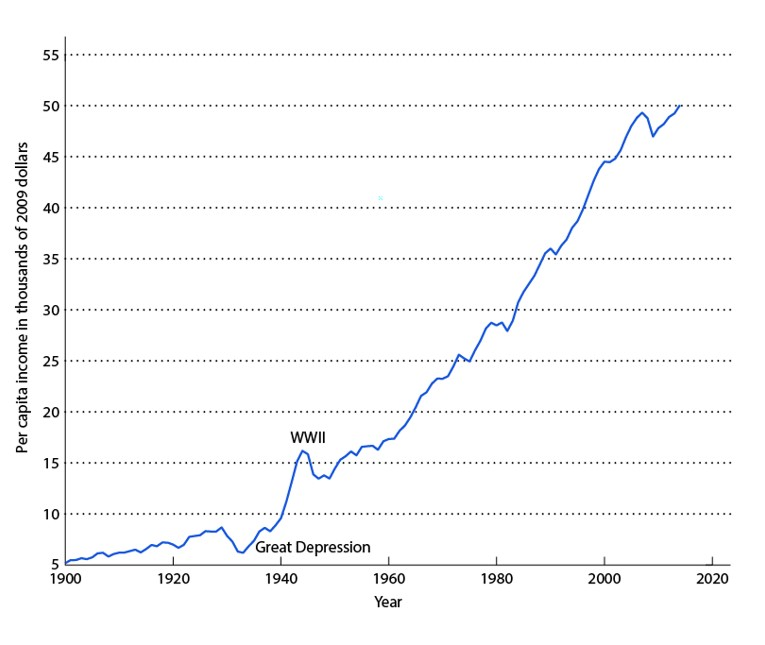
\includegraphics[width=\textwidth]{./figures/Figure1_1.jpg}
            \end{figure}
        \end{column}
        \begin{column}{0.5\textwidth}
            \begin{figure}
                \caption{Figure 1.3: Natural log of Per Capita Real GDP and trend, 1900–2014 (Trend: HP Filter)}
                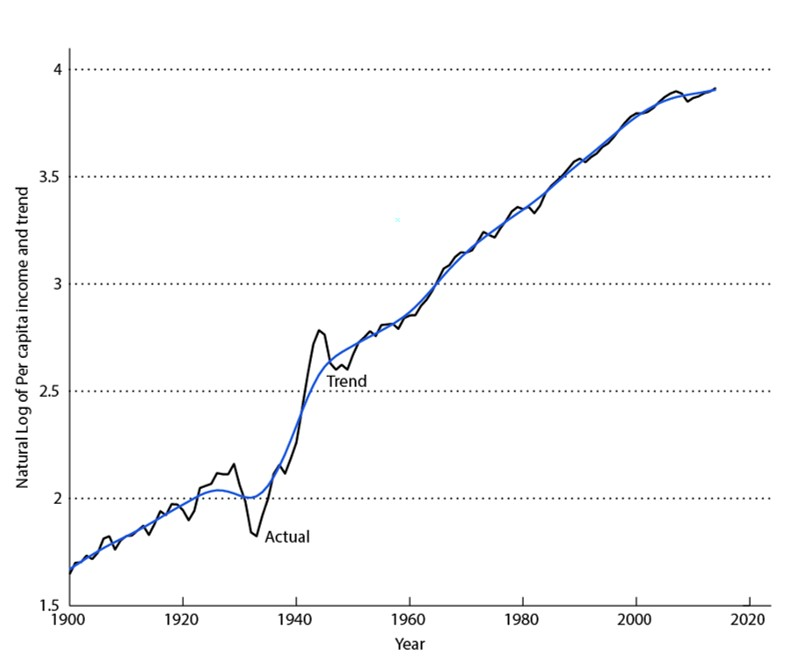
\includegraphics[width=\textwidth]{./figures/Figure1_3.jpg}
            \end{figure}
        \end{column}
    \end{columns}
\end{frame}

\begin{frame}{Business Cycle: Deviation from Trend}
\label{slide:Business_Cycle__Deviation_from_Trend}
    \begin{columns}
        \begin{column}{0.5\textwidth}
            \begin{figure}
                \caption{Figure 1.4 Percentage Deviation from Trend in Per Capita Real GDP, \alert{actual - trend}}
                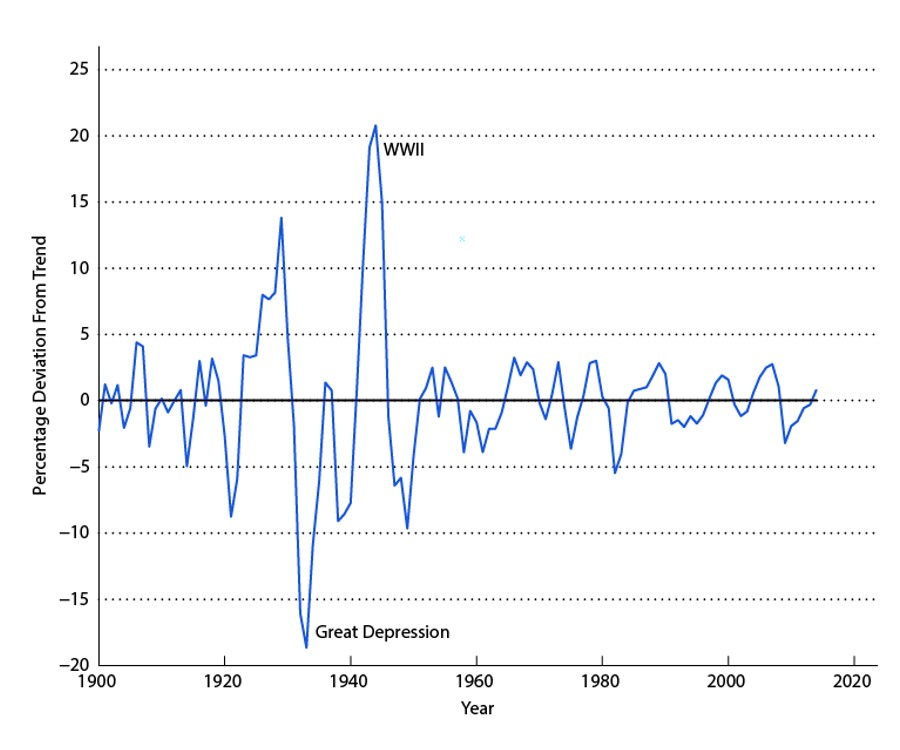
\includegraphics[width=\textwidth]{./figures/Figure1_4.jpg}
            \end{figure}
        \end{column}
        \begin{column}{0.5\textwidth}
            \begin{figure}
                \caption{Figure 1.13 Percentage Deviation From Trend in Real GDP, \alert{same transform as 1.1, 1.3, 1.4, not per capita} }
                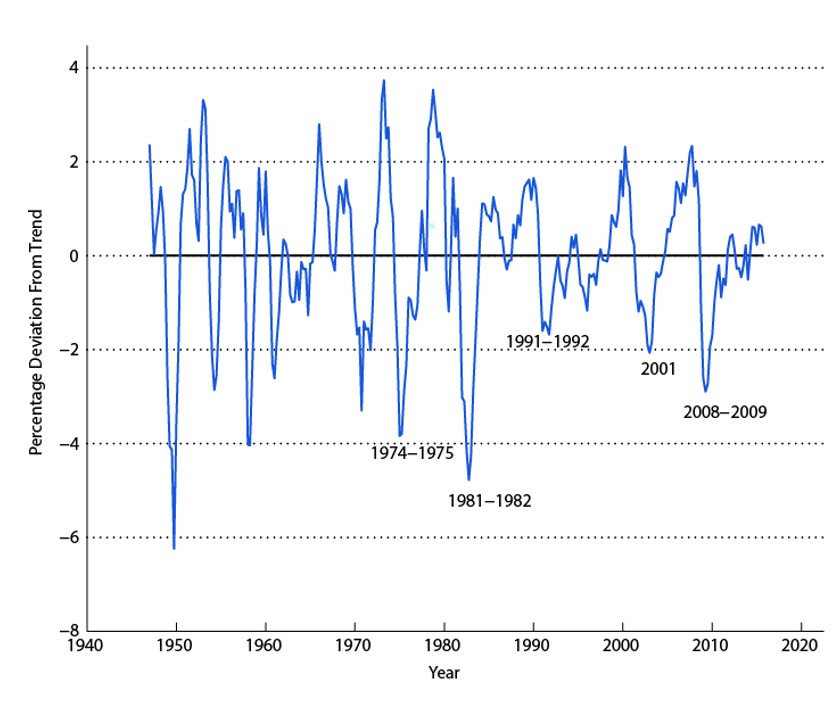
\includegraphics[width=\textwidth]{./figures/Figure1_13.jpg}
            \end{figure}
        \end{column}
    \end{columns}
\end{frame}

\begin{frame}{Using Macro Model to Understand Data}
\label{slide:Using_Macro_Model_to_Understand_Data}
    \begin{itemize}
        \item Economics is a \alert{scientific pursuit} involving the formulation and \alert{refinement of theories} that can help us better understand \alert{how economies work} and \alert{how they can be improved}
        \item \textbf{Data}: \alert{how economies work}, e.g. GDP example
        \item \textbf{Theory}: cannot do experiment at economy scale $ \Rightarrow  $ only way for \alert{scientific pursuit}
        \item \textbf{Policy}: understand \alert{how economies can be improved} by \alert{policies}
    \end{itemize}
\end{frame}

\begin{frame}{Anecdotic Illustration of Economics Model}
\label{slide:Anecdotic_Illustration_of_Economics_Model}

\begin{center}
Build your own world (similar to real world) so that you know every detail!

\includegraphics[width=0.8\textwidth]{./figures/6375692be499513c6f3be825_Minecraft-logo.png}
\end{center}

\end{frame}

\begin{frame}{Structure of Macro Model: $ 4 $ elements}
\label{slide:Structure_of_Macro_Model____4___elements}
\begin{enumerate}
    \item \textbf{Agent}: who is involved?
    \begin{itemize}
        \item e.g. consumers, firms, governments, etc.
    \end{itemize}
    \item \textbf{Preferences}: how and what is consumed/valued/invested?
    \begin{itemize}
        \item e.g. consumers' utility function on goods
    \end{itemize}
    \item \textbf{Resources}: availability and distribution
    \begin{itemize}
        \item e.g. Wealth, time, talents, natural resources
    \end{itemize}
    \item \textbf{Technology}: objective limitation at given period of time
    \begin{itemize}
        \item firms' production, market structure
    \end{itemize}
\end{enumerate}
\end{frame}

\begin{frame}{Analysis on Macro Model: $ 3 $ steps}
\label{slide:Analysis_on_Macro_Model____3___steps}
    \begin{enumerate}
        \item \textbf{Equilibrium}: how do all the forces balanced?
        \begin{itemize}
            \item e.g. competitive equilibrium
        \end{itemize}
        \item \textbf{Assessment}: what's model prediction, and how different from data?
        \begin{itemize}
            \item relationship between consumption and output
        \end{itemize}
        \item \textbf{Refinement}: how do changes in model alter its prediction?
        \begin{itemize}
            \item different technology, one-period $ \rightarrow  $ two-period
        \end{itemize}
    \end{enumerate}
\end{frame}

\begin{frame}{What makes a good model?}
\label{slide:What_makes_a_good_model_}
    \begin{center}
        \alert{Friedman's critique}: models are judged by \alert{prediction power}
    \end{center}
    \begin{itemize}
        \item Clarity: is the logic and causality understandable?
        \item Prediction power: match data?
        \item Communication: what we (dis-)agree about?
    \end{itemize}

    \vspace{0.7em}

    ALL models are fake, only some are useful, i.e., elucidates the \alert{underlying mechanism} that people implicitly follows

\end{frame}


\begin{frame}{Just Micro?}
\label{slide:Just_Micro_}
    \alert{Yes!} Macro models need micro-foundation, because
    \begin{itemize}
        \item aggregate behavior is the sum of individual decisions
        \item \alert{Lucas' critique}: structures of economies \alert{change} w/ policies b/c \alert{individual decision} changed
        \item Need to know effect on \alert{individual behavior} to know the aggregate effect!
        \item E.g. Two force of COVID stimulus policy:
        \begin{enumerate}
            \item $ \Rightarrow  $ workers have \alert{less} incentive to work $ \Rightarrow  $ unemployment $ \uparrow  $ $ \Rightarrow  $ exacerbate recession
            \item $ \Rightarrow  $ funding $ \uparrow  $ $ \Rightarrow  $ firms have \alert{more} incentive to hire workers $ \Rightarrow  $ mitigate recession
        \end{enumerate}
    \end{itemize}
\end{frame}

\appendix

% \begin{frame}[allowframebreaks]{References}
% \footnotesize
% \bibliographystyle{$BIB_STYLE}
% \bibliography{$BIBFILE}
% \end{frame}

\end{document}
